\documentclass{article}

\usepackage{listings}
\usepackage{amsmath}
\usepackage{graphicx}
\usepackage{hyperref}
\usepackage{booktabs}
\usepackage{verbatim}
\usepackage{url}

\begin{document}

\title{Homework 8\\
       Part B and C}
\author{Geoffrey Ulman\\
        CSI740}
\date{April 2012}
\maketitle

\section{Problem Statement}\label{prob}

Consider the linear system \(Ax=b\) where \(A\) and \(b\) are defined in Equation \ref{eq1}.

\begin{equation}
A =
  \begin{bmatrix}
    1 & 1 + \epsilon \\
    1 - 2\epsilon & 1 \\
  \end{bmatrix}
\hspace{.2in}
b = 
  \begin{bmatrix}
    1 \\
    0 \\
  \end{bmatrix}
\label{eq1}
\end{equation}

\section{Condition Number}\label{cond}

Solutions for Equation \ref{eq1} were calculated for \( \epsilon \) values from the set \( \{2^k\epsilon_{Machine}:\text{$k$ = 0..52}\} \). For IEEE Double Precision values, this is approximately from \( \epsilon_{Machine} \) to 1. The condition number for the 2 norm of the matrix A is plotted for all tested \( \epsilon \) values in Figure \ref{plot1}. As expected, the condition numbers calculated by Matlab for other norms were of approximately the same order of magnitude.

\section{Solution Error}\label{error}

Although the matrix condition number behaved as expected, the relative error between the exact and Matlab calculated values of \(x\) behaved counter-intuitively. The relative error of x as a function of \( \epsilon \) is plotted in Figure \ref{plot2}. As \( \epsilon \) approaches approximately \(10^{-8}\), the relative error increases (which is unexpected because the condition number of A is decreasing on this interval. Further, past \(10^{-8}\) the relative error drops to essentially 0.

This is partially explained by the absolute error of x, shown in Figure \ref{plot4}, and the 2-norm of x, shown in Figure \ref{plot5}. The calculated absolute error is essentially constant from \(\epsilon=10^{-16}\) to \(\epsilon=10^{-8}\), then drops to near 0. The 2-norm of x starts extremely large (which is expected given the near-signular nature of the matrix \(A\)) and drops to 0 near \( \epsilon = 1 \). This means that decreasing relative error of \(x\) is driven by the decreasing 2-norm of \(x\) on \(\epsilon=10^{-16}\) to \(\epsilon=10^{-8}\).

It is, however, possible that this result is a result of catestophic cancellation or numeric error by the calculations used to compare they extremely large calculated and exact \(x\) values.

\section{Other Norms}\label{norms}

The only effect using norms besides the 2-norm had on the above calculations was to change the value of the condition number of A (but not the magnitude of the values). Changing norms also changed the height of the plateau observed in the absolute error in Figure \ref{plot4}, but all the plots displayed the same qualitative behavior.

\begin{figure}
\centering
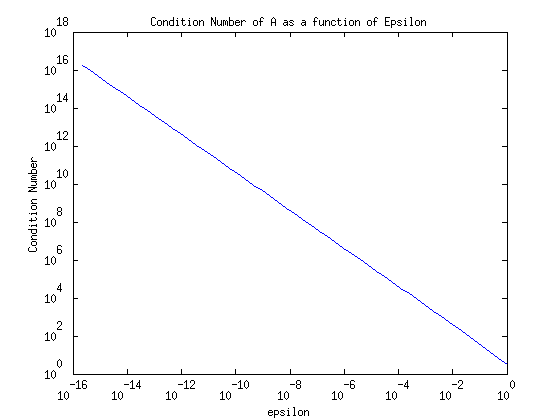
\includegraphics[width=1.0\textwidth]{plot1.png}
\caption{Condition Number of A as a function of Epsilon}
\label{plot1}
\end{figure}

\begin{figure}
\centering
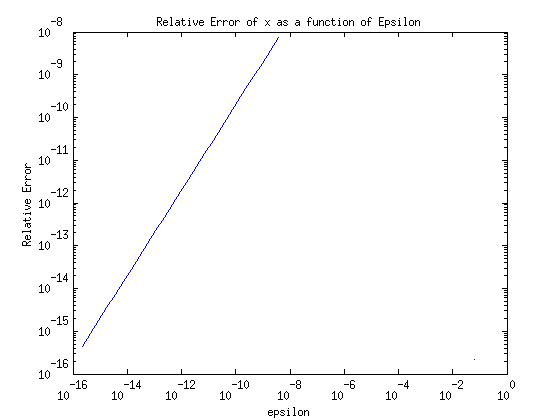
\includegraphics[width=1.0\textwidth]{plot2.png}
\caption{Relative Error of x as a function of Epsilon}
\label{plot2}
\end{figure}

\begin{figure}
\centering
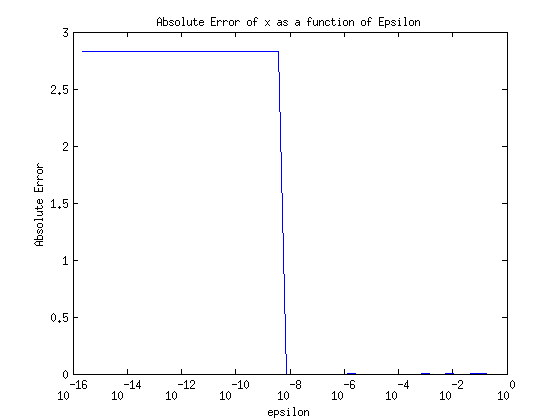
\includegraphics[width=1.0\textwidth]{plot4.png}
\caption{Absolute Error of x as a function of Epsilon}
\label{plot4}
\end{figure}

\begin{figure}
\centering
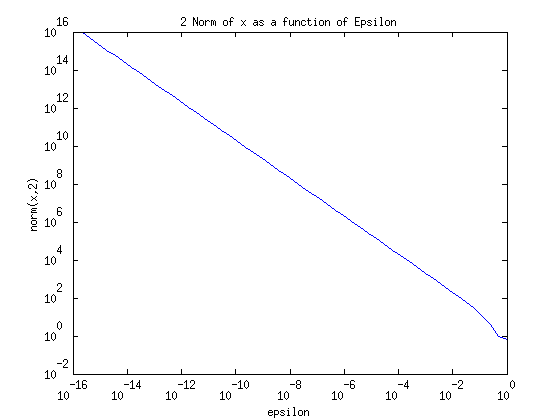
\includegraphics[width=1.0\textwidth]{plot5.png}
\caption{2-Norm of x as a function of Epsilon}
\label{plot5}
\end{figure}

\end{document}
